% Options for packages loaded elsewhere
% Options for packages loaded elsewhere
\PassOptionsToPackage{unicode}{hyperref}
\PassOptionsToPackage{hyphens}{url}
\PassOptionsToPackage{dvipsnames,svgnames,x11names}{xcolor}
%
\documentclass[
  letterpaper,
  DIV=11,
  numbers=noendperiod]{scrartcl}
\usepackage{xcolor}
\usepackage{amsmath,amssymb}
\setcounter{secnumdepth}{-\maxdimen} % remove section numbering
\usepackage{iftex}
\ifPDFTeX
  \usepackage[T1]{fontenc}
  \usepackage[utf8]{inputenc}
  \usepackage{textcomp} % provide euro and other symbols
\else % if luatex or xetex
  \usepackage{unicode-math} % this also loads fontspec
  \defaultfontfeatures{Scale=MatchLowercase}
  \defaultfontfeatures[\rmfamily]{Ligatures=TeX,Scale=1}
\fi
\usepackage{lmodern}
\ifPDFTeX\else
  % xetex/luatex font selection
\fi
% Use upquote if available, for straight quotes in verbatim environments
\IfFileExists{upquote.sty}{\usepackage{upquote}}{}
\IfFileExists{microtype.sty}{% use microtype if available
  \usepackage[]{microtype}
  \UseMicrotypeSet[protrusion]{basicmath} % disable protrusion for tt fonts
}{}
\makeatletter
\@ifundefined{KOMAClassName}{% if non-KOMA class
  \IfFileExists{parskip.sty}{%
    \usepackage{parskip}
  }{% else
    \setlength{\parindent}{0pt}
    \setlength{\parskip}{6pt plus 2pt minus 1pt}}
}{% if KOMA class
  \KOMAoptions{parskip=half}}
\makeatother
% Make \paragraph and \subparagraph free-standing
\makeatletter
\ifx\paragraph\undefined\else
  \let\oldparagraph\paragraph
  \renewcommand{\paragraph}{
    \@ifstar
      \xxxParagraphStar
      \xxxParagraphNoStar
  }
  \newcommand{\xxxParagraphStar}[1]{\oldparagraph*{#1}\mbox{}}
  \newcommand{\xxxParagraphNoStar}[1]{\oldparagraph{#1}\mbox{}}
\fi
\ifx\subparagraph\undefined\else
  \let\oldsubparagraph\subparagraph
  \renewcommand{\subparagraph}{
    \@ifstar
      \xxxSubParagraphStar
      \xxxSubParagraphNoStar
  }
  \newcommand{\xxxSubParagraphStar}[1]{\oldsubparagraph*{#1}\mbox{}}
  \newcommand{\xxxSubParagraphNoStar}[1]{\oldsubparagraph{#1}\mbox{}}
\fi
\makeatother

\usepackage{color}
\usepackage{fancyvrb}
\newcommand{\VerbBar}{|}
\newcommand{\VERB}{\Verb[commandchars=\\\{\}]}
\DefineVerbatimEnvironment{Highlighting}{Verbatim}{commandchars=\\\{\}}
% Add ',fontsize=\small' for more characters per line
\usepackage{framed}
\definecolor{shadecolor}{RGB}{241,243,245}
\newenvironment{Shaded}{\begin{snugshade}}{\end{snugshade}}
\newcommand{\AlertTok}[1]{\textcolor[rgb]{0.68,0.00,0.00}{#1}}
\newcommand{\AnnotationTok}[1]{\textcolor[rgb]{0.37,0.37,0.37}{#1}}
\newcommand{\AttributeTok}[1]{\textcolor[rgb]{0.40,0.45,0.13}{#1}}
\newcommand{\BaseNTok}[1]{\textcolor[rgb]{0.68,0.00,0.00}{#1}}
\newcommand{\BuiltInTok}[1]{\textcolor[rgb]{0.00,0.23,0.31}{#1}}
\newcommand{\CharTok}[1]{\textcolor[rgb]{0.13,0.47,0.30}{#1}}
\newcommand{\CommentTok}[1]{\textcolor[rgb]{0.37,0.37,0.37}{#1}}
\newcommand{\CommentVarTok}[1]{\textcolor[rgb]{0.37,0.37,0.37}{\textit{#1}}}
\newcommand{\ConstantTok}[1]{\textcolor[rgb]{0.56,0.35,0.01}{#1}}
\newcommand{\ControlFlowTok}[1]{\textcolor[rgb]{0.00,0.23,0.31}{\textbf{#1}}}
\newcommand{\DataTypeTok}[1]{\textcolor[rgb]{0.68,0.00,0.00}{#1}}
\newcommand{\DecValTok}[1]{\textcolor[rgb]{0.68,0.00,0.00}{#1}}
\newcommand{\DocumentationTok}[1]{\textcolor[rgb]{0.37,0.37,0.37}{\textit{#1}}}
\newcommand{\ErrorTok}[1]{\textcolor[rgb]{0.68,0.00,0.00}{#1}}
\newcommand{\ExtensionTok}[1]{\textcolor[rgb]{0.00,0.23,0.31}{#1}}
\newcommand{\FloatTok}[1]{\textcolor[rgb]{0.68,0.00,0.00}{#1}}
\newcommand{\FunctionTok}[1]{\textcolor[rgb]{0.28,0.35,0.67}{#1}}
\newcommand{\ImportTok}[1]{\textcolor[rgb]{0.00,0.46,0.62}{#1}}
\newcommand{\InformationTok}[1]{\textcolor[rgb]{0.37,0.37,0.37}{#1}}
\newcommand{\KeywordTok}[1]{\textcolor[rgb]{0.00,0.23,0.31}{\textbf{#1}}}
\newcommand{\NormalTok}[1]{\textcolor[rgb]{0.00,0.23,0.31}{#1}}
\newcommand{\OperatorTok}[1]{\textcolor[rgb]{0.37,0.37,0.37}{#1}}
\newcommand{\OtherTok}[1]{\textcolor[rgb]{0.00,0.23,0.31}{#1}}
\newcommand{\PreprocessorTok}[1]{\textcolor[rgb]{0.68,0.00,0.00}{#1}}
\newcommand{\RegionMarkerTok}[1]{\textcolor[rgb]{0.00,0.23,0.31}{#1}}
\newcommand{\SpecialCharTok}[1]{\textcolor[rgb]{0.37,0.37,0.37}{#1}}
\newcommand{\SpecialStringTok}[1]{\textcolor[rgb]{0.13,0.47,0.30}{#1}}
\newcommand{\StringTok}[1]{\textcolor[rgb]{0.13,0.47,0.30}{#1}}
\newcommand{\VariableTok}[1]{\textcolor[rgb]{0.07,0.07,0.07}{#1}}
\newcommand{\VerbatimStringTok}[1]{\textcolor[rgb]{0.13,0.47,0.30}{#1}}
\newcommand{\WarningTok}[1]{\textcolor[rgb]{0.37,0.37,0.37}{\textit{#1}}}

\usepackage{longtable,booktabs,array}
\newcounter{none} % for unnumbered tables
\usepackage{calc} % for calculating minipage widths
% Correct order of tables after \paragraph or \subparagraph
\usepackage{etoolbox}
\makeatletter
\patchcmd\longtable{\par}{\if@noskipsec\mbox{}\fi\par}{}{}
\makeatother
% Allow footnotes in longtable head/foot
\IfFileExists{footnotehyper.sty}{\usepackage{footnotehyper}}{\usepackage{footnote}}
\makesavenoteenv{longtable}
\usepackage{graphicx}
\makeatletter
\newsavebox\pandoc@box
\newcommand*\pandocbounded[1]{% scales image to fit in text height/width
  \sbox\pandoc@box{#1}%
  \Gscale@div\@tempa{\textheight}{\dimexpr\ht\pandoc@box+\dp\pandoc@box\relax}%
  \Gscale@div\@tempb{\linewidth}{\wd\pandoc@box}%
  \ifdim\@tempb\p@<\@tempa\p@\let\@tempa\@tempb\fi% select the smaller of both
  \ifdim\@tempa\p@<\p@\scalebox{\@tempa}{\usebox\pandoc@box}%
  \else\usebox{\pandoc@box}%
  \fi%
}
% Set default figure placement to htbp
\def\fps@figure{htbp}
\makeatother





\setlength{\emergencystretch}{3em} % prevent overfull lines

\providecommand{\tightlist}{%
  \setlength{\itemsep}{0pt}\setlength{\parskip}{0pt}}



 


\KOMAoption{captions}{tableheading}
\makeatletter
\@ifpackageloaded{caption}{}{\usepackage{caption}}
\AtBeginDocument{%
\ifdefined\contentsname
  \renewcommand*\contentsname{Table of contents}
\else
  \newcommand\contentsname{Table of contents}
\fi
\ifdefined\listfigurename
  \renewcommand*\listfigurename{List of Figures}
\else
  \newcommand\listfigurename{List of Figures}
\fi
\ifdefined\listtablename
  \renewcommand*\listtablename{List of Tables}
\else
  \newcommand\listtablename{List of Tables}
\fi
\ifdefined\figurename
  \renewcommand*\figurename{Figure}
\else
  \newcommand\figurename{Figure}
\fi
\ifdefined\tablename
  \renewcommand*\tablename{Table}
\else
  \newcommand\tablename{Table}
\fi
}
\@ifpackageloaded{float}{}{\usepackage{float}}
\floatstyle{ruled}
\@ifundefined{c@chapter}{\newfloat{codelisting}{h}{lop}}{\newfloat{codelisting}{h}{lop}[chapter]}
\floatname{codelisting}{Listing}
\newcommand*\listoflistings{\listof{codelisting}{List of Listings}}
\makeatother
\makeatletter
\makeatother
\makeatletter
\@ifpackageloaded{caption}{}{\usepackage{caption}}
\@ifpackageloaded{subcaption}{}{\usepackage{subcaption}}
\makeatother
\usepackage{bookmark}
\IfFileExists{xurl.sty}{\usepackage{xurl}}{} % add URL line breaks if available
\urlstyle{same}
\hypersetup{
  pdftitle={ENVS 193DS Homework 3},
  pdfauthor={Danielle Sur},
  colorlinks=true,
  linkcolor={blue},
  filecolor={Maroon},
  citecolor={Blue},
  urlcolor={Blue},
  pdfcreator={LaTeX via pandoc}}


\title{ENVS 193DS Homework 3}
\author{Danielle Sur}
\date{2026-05-31}
\begin{document}
\maketitle

\renewcommand*\contentsname{Table of contents}
{
\setcounter{tocdepth}{3}
\tableofcontents
}

\section{Set up}\label{set-up}

\begin{Shaded}
\begin{Highlighting}[]
\CommentTok{\# loaded in packages}
\FunctionTok{library}\NormalTok{(tidyverse)}
\FunctionTok{library}\NormalTok{(janitor)}
\FunctionTok{library}\NormalTok{(here)}
\FunctionTok{library}\NormalTok{(readxl)}

\CommentTok{\# read in data and saved as object called \textasciigrave{}kelp\textasciigrave{}}
\NormalTok{kelp   }\OtherTok{\textless{}{-}}\NormalTok{ readr}\SpecialCharTok{::}\FunctionTok{read\_csv}\NormalTok{(here}\SpecialCharTok{::}\FunctionTok{here}\NormalTok{(}\StringTok{"data"}\NormalTok{,}\StringTok{"temp{-}kelp.csv"}\NormalTok{))}
\CommentTok{\# read in my data and saved as object called \textquotesingle{}rxntime\textquotesingle{}}
\NormalTok{rxntime }\OtherTok{\textless{}{-}}\NormalTok{ readr}\SpecialCharTok{::}\FunctionTok{read\_csv}\NormalTok{(here}\SpecialCharTok{::}\FunctionTok{here}\NormalTok{(}\StringTok{"data"}\NormalTok{,}\StringTok{"rxn{-}time.csv"}\NormalTok{))}
\end{Highlighting}
\end{Shaded}

\section{Problem 1. Giant kelp
fronds}\label{problem-1.-giant-kelp-fronds}

\subsection{a. An appropriate test}\label{a.-an-appropriate-test}

Pearson's correlation and ordinary least squares can be used to test the
strength of the relationship between temperature and giant kelp frond
elongation rate. Whereas Pearson's r would indicate the strength and
direction of linear association between the two variables (temperature
and kelp elongation rate), the OLS slope would predict changes in the
response variable (kelp elongation rate) based on the value of the
predictor variable (temperature) and can account for multiple variables.

\subsection{b. Create a visualization}\label{b.-create-a-visualization}

\begin{Shaded}
\begin{Highlighting}[]
\CommentTok{\# base layer: ggplot}
\FunctionTok{ggplot}\NormalTok{(kelp,}
       \CommentTok{\# x{-}axis: temperature}
       \CommentTok{\# y{-}axis: kelp elongation}
       \FunctionTok{aes}\NormalTok{(}\AttributeTok{x =}\NormalTok{ temp\_c,}
           \AttributeTok{y =}\NormalTok{ kelp\_elong)) }\SpecialCharTok{+}
  \CommentTok{\# added raw data points with custom color}
  \FunctionTok{geom\_point}\NormalTok{(}\AttributeTok{color =} \StringTok{"dodgerblue"}\NormalTok{) }\SpecialCharTok{+}
  \CommentTok{\# fitted a linear model}
  \FunctionTok{geom\_smooth}\NormalTok{(}\AttributeTok{method =} \StringTok{"lm"}\NormalTok{, }\AttributeTok{se =} \ConstantTok{TRUE}\NormalTok{) }\SpecialCharTok{+}
  \CommentTok{\# relabeled x and y axes}
  \FunctionTok{labs}\NormalTok{(}\AttributeTok{x =} \StringTok{"Temperature (°C)"}\NormalTok{,}
       \AttributeTok{y =} \StringTok{"Kelp Elongation (cm/day)"}\NormalTok{) }\SpecialCharTok{+}
  \CommentTok{\# changed default theme}
  \FunctionTok{theme\_minimal}\NormalTok{()}
\end{Highlighting}
\end{Shaded}

\pandocbounded{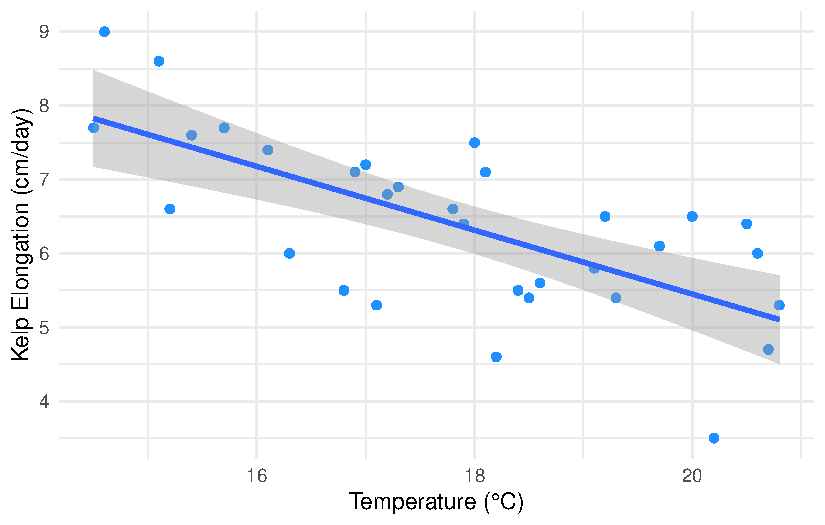
\includegraphics[keepaspectratio]{ENVS-193DS_homework-3_files/figure-pdf/unnamed-chunk-2-1.pdf}}

\subsection{c.~Check your assumptions and run your
test}\label{c.-check-your-assumptions-and-run-your-test}

\subsubsection{Check your assumptions}\label{check-your-assumptions}

\begin{Shaded}
\begin{Highlighting}[]
\CommentTok{\# fitted model}
\NormalTok{kelp\_model }\OtherTok{\textless{}{-}} \FunctionTok{lm}\NormalTok{(}
\NormalTok{  kelp\_elong }\SpecialCharTok{\textasciitilde{}}\NormalTok{ temp\_c,}
  \AttributeTok{data =}\NormalTok{ kelp)}

\CommentTok{\# model information}
\FunctionTok{summary}\NormalTok{(kelp\_model)}
\end{Highlighting}
\end{Shaded}

\begin{verbatim}

Call:
lm(formula = kelp_elong ~ temp_c, data = kelp)

Residuals:
    Min      1Q  Median      3Q     Max 
-1.8643 -0.5017  0.1790  0.5659  1.2177 

Coefficients:
            Estimate Std. Error t value Pr(>|t|)    
(Intercept) 14.08645    1.49219   9.440 1.72e-10 ***
temp_c      -0.43179    0.08321  -5.189 1.37e-05 ***
---
Signif. codes:  0 '***' 0.001 '**' 0.01 '*' 0.05 '.' 0.1 ' ' 1

Residual standard error: 0.8665 on 30 degrees of freedom
Multiple R-squared:  0.473, Adjusted R-squared:  0.4554 
F-statistic: 26.93 on 1 and 30 DF,  p-value: 1.366e-05
\end{verbatim}

\begin{Shaded}
\begin{Highlighting}[]
\CommentTok{\# base R residuals}
\FunctionTok{par}\NormalTok{(}\AttributeTok{mfrow =} \FunctionTok{c}\NormalTok{(}\DecValTok{2}\NormalTok{,}\DecValTok{2}\NormalTok{))}
\FunctionTok{plot}\NormalTok{(kelp\_model)}
\end{Highlighting}
\end{Shaded}

\pandocbounded{\includegraphics[keepaspectratio]{ENVS-193DS_homework-3_files/figure-pdf/unnamed-chunk-4-1.pdf}}

\begin{Shaded}
\begin{Highlighting}[]
\CommentTok{\# Pearson\textquotesingle{}s correlation test}
\FunctionTok{cor.test}\NormalTok{(kelp}\SpecialCharTok{$}\NormalTok{temp\_c, kelp}\SpecialCharTok{$}\NormalTok{kelp\_elong,}
         \AttributeTok{method =} \StringTok{"pearson"}\NormalTok{)}
\end{Highlighting}
\end{Shaded}

\begin{verbatim}

    Pearson's product-moment correlation

data:  kelp$temp_c and kelp$kelp_elong
t = -5.189, df = 30, p-value = 1.366e-05
alternative hypothesis: true correlation is not equal to 0
95 percent confidence interval:
 -0.8359665 -0.4460157
sample estimates:
       cor 
-0.6877489 
\end{verbatim}

I checked that there was a linear relationship between variables (). I
also checked that errors were independent of each other (),
homoscedastic (), and normally distributed.

\subsubsection{Run test}\label{run-test}

\subsection{d.~Results communication}\label{d.-results-communication}

\subsection{e. Test implications}\label{e.-test-implications}

\subsection{f.~Double check your own
work}\label{f.-double-check-your-own-work}

\section{Problem 2. Personal data}\label{problem-2.-personal-data}

\subsection{a. Updating your
visualizations}\label{a.-updating-your-visualizations}

\subsubsection{Cleaning data}\label{cleaning-data}

\begin{Shaded}
\begin{Highlighting}[]
\CommentTok{\# created a new object from rxntime}
\NormalTok{rxntime\_type }\OtherTok{\textless{}{-}}\NormalTok{ rxntime }\SpecialCharTok{|\textgreater{}} 
  \CommentTok{\# cleaned column names}
 \FunctionTok{clean\_names}\NormalTok{() }\SpecialCharTok{|\textgreater{}} 
  \CommentTok{\# selected columns of interest}
  \FunctionTok{select}\NormalTok{(exercise\_type, reaction\_time\_avg\_ms) }\SpecialCharTok{|\textgreater{}} 
  \CommentTok{\# removed missing values}
  \FunctionTok{drop\_na}\NormalTok{(exercise\_type, reaction\_time\_avg\_ms) }\SpecialCharTok{|\textgreater{}} 
  \CommentTok{\# capitalized existing exercise type categories}
  \FunctionTok{mutate}\NormalTok{(}\AttributeTok{exercise\_type =} \FunctionTok{case\_when}\NormalTok{(}
\NormalTok{    exercise\_type }\SpecialCharTok{==} \StringTok{"biking"} \SpecialCharTok{\textasciitilde{}} \StringTok{"Biking"}\NormalTok{,}
\NormalTok{    exercise\_type }\SpecialCharTok{==} \StringTok{"volleyball"} \SpecialCharTok{\textasciitilde{}} \StringTok{"Volleyball"}\NormalTok{,}
\NormalTok{    exercise\_type }\SpecialCharTok{==} \StringTok{"walking"} \SpecialCharTok{\textasciitilde{}} \StringTok{"Walking"}
\NormalTok{  ))}
\end{Highlighting}
\end{Shaded}

\begin{Shaded}
\begin{Highlighting}[]
\CommentTok{\# created a new object from rxntime}
\NormalTok{rxntime\_clean }\OtherTok{\textless{}{-}}\NormalTok{ rxntime }\SpecialCharTok{|\textgreater{}} 
  \CommentTok{\# cleaned column names}
 \FunctionTok{clean\_names}\NormalTok{() }\SpecialCharTok{|\textgreater{}} 
  \CommentTok{\# selected columns of interest}
  \FunctionTok{select}\NormalTok{(exercise\_duration\_min, reaction\_time\_avg\_ms) }\SpecialCharTok{|\textgreater{}}
  \CommentTok{\# removed missing values}
  \FunctionTok{drop\_na}\NormalTok{(exercise\_duration\_min, reaction\_time\_avg\_ms)}
\end{Highlighting}
\end{Shaded}

\subsubsection{Figure 1. Exercise type and reaction
time}\label{figure-1.-exercise-type-and-reaction-time}

\begin{Shaded}
\begin{Highlighting}[]
\CommentTok{\# base layer: ggplot}
\FunctionTok{ggplot}\NormalTok{(}\AttributeTok{data =}\NormalTok{ rxntime\_type,}
       \CommentTok{\# x{-}axis: exercise type}
       \CommentTok{\# y{-}axis: average reaction time in milliseconds}
       \CommentTok{\# color by exercise type}
       \AttributeTok{mapping =} \FunctionTok{aes}\NormalTok{(}\AttributeTok{x =} \StringTok{"Exercise Type"}\NormalTok{,}
                     \AttributeTok{y =} \StringTok{"Average Reaction Time (ms)"}\NormalTok{,}
                     \AttributeTok{color =}\NormalTok{ exercise\_type)) }\SpecialCharTok{+}
  \CommentTok{\# first layer: data points}
  \FunctionTok{geom\_point}\NormalTok{(}\AttributeTok{data =}\NormalTok{ rxntime\_type,}
             \FunctionTok{aes}\NormalTok{(}\AttributeTok{x =}\NormalTok{ exercise\_type,}
                 \AttributeTok{y =}\NormalTok{ reaction\_time\_avg\_ms,}
                 \AttributeTok{size =} \DecValTok{3}\NormalTok{)) }\SpecialCharTok{+}
  \CommentTok{\# changed theme}
  \FunctionTok{theme\_minimal}\NormalTok{() }\SpecialCharTok{+}
  \CommentTok{\# removed legend}
  \FunctionTok{theme}\NormalTok{(}\AttributeTok{legend.position =} \StringTok{"none"}\NormalTok{,}
        \AttributeTok{panel.background =} \FunctionTok{element\_blank}\NormalTok{(), }\CommentTok{\# removing panel background}
        \AttributeTok{panel.grid =} \FunctionTok{element\_blank}\NormalTok{(), }\CommentTok{\# removing panel grid}
        \AttributeTok{axis.ticks =} \FunctionTok{element\_blank}\NormalTok{() }\CommentTok{\# removing axis ticks)}
\NormalTok{  ) }\SpecialCharTok{+}
  \CommentTok{\# relabeled x{-} and y{-} axes, adding title}
  \FunctionTok{labs}\NormalTok{(}\AttributeTok{title =} \StringTok{"Exercise Type and Reaction Time"}\NormalTok{,}
       \AttributeTok{subtitle =} \StringTok{"May 29, 2026"}\NormalTok{,}
       \AttributeTok{x =} \StringTok{"Exercise Type"}\NormalTok{,}
       \AttributeTok{y =} \StringTok{"Average Reaction Time (ms)"}\NormalTok{) }\SpecialCharTok{+}
  \CommentTok{\# custom colors}
  \FunctionTok{scale\_color\_manual}\NormalTok{(}\AttributeTok{values =}
                       \FunctionTok{c}\NormalTok{(}\StringTok{"Biking"} \OtherTok{=} \StringTok{"magenta"}\NormalTok{,}
                         \StringTok{"Volleyball"} \OtherTok{=} \StringTok{"purple3"}\NormalTok{,}
                         \StringTok{"Walking"} \OtherTok{=} \StringTok{"blue"}\NormalTok{))}
\end{Highlighting}
\end{Shaded}

\pandocbounded{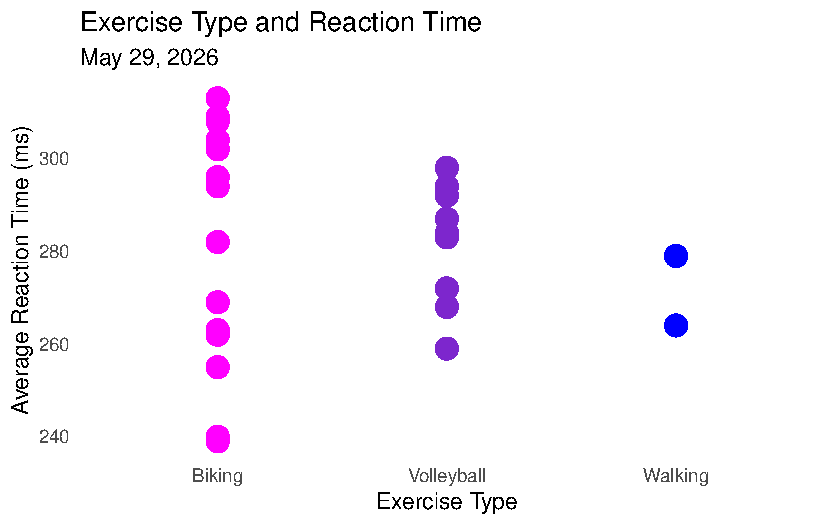
\includegraphics[keepaspectratio]{ENVS-193DS_homework-3_files/figure-pdf/unnamed-chunk-8-1.pdf}}

\subsubsection{Figure 2. Exercise duration and reaction
time}\label{figure-2.-exercise-duration-and-reaction-time}

\begin{Shaded}
\begin{Highlighting}[]
\CommentTok{\# base layer: ggplot}
\FunctionTok{ggplot}\NormalTok{(}\AttributeTok{data =}\NormalTok{ rxntime\_clean,}
       \CommentTok{\# x{-}axis: exercise duration in minutes}
       \CommentTok{\# y{-}axis: average reaction time in milliseconds}
       \CommentTok{\# color}
       \AttributeTok{mapping =} \FunctionTok{aes}\NormalTok{(}\AttributeTok{x =} \StringTok{"Exercise Type"}\NormalTok{,}
                     \AttributeTok{y =} \StringTok{"Average Reaction Time (ms)"}\NormalTok{)) }\SpecialCharTok{+}
  \CommentTok{\# first layer: data points}
  \FunctionTok{geom\_point}\NormalTok{(}\AttributeTok{data =}\NormalTok{ rxntime\_clean,}
             \FunctionTok{aes}\NormalTok{(}\AttributeTok{x =}\NormalTok{ exercise\_duration\_min,}
                 \AttributeTok{y =}\NormalTok{ reaction\_time\_avg\_ms,}
                 \AttributeTok{size =} \DecValTok{3}\NormalTok{,}
                 \AttributeTok{color =} \StringTok{"hotpink"}\NormalTok{)) }\SpecialCharTok{+}
  \CommentTok{\# changed theme}
  \FunctionTok{theme\_minimal}\NormalTok{() }\SpecialCharTok{+}
  \CommentTok{\# removed legend}
  \FunctionTok{theme}\NormalTok{(}\AttributeTok{legend.position =} \StringTok{"none"}\NormalTok{,}
        \AttributeTok{panel.background =} \FunctionTok{element\_blank}\NormalTok{(), }\CommentTok{\# removing panel background}
        \AttributeTok{panel.grid =} \FunctionTok{element\_blank}\NormalTok{(), }\CommentTok{\# removing panel grid}
        \AttributeTok{axis.ticks =} \FunctionTok{element\_blank}\NormalTok{(), }\CommentTok{\# removing axis ticks}
\NormalTok{    ) }\SpecialCharTok{+}
  \CommentTok{\# relabeled x{-} and y{-} axes, adding title}
  \FunctionTok{labs}\NormalTok{(}\AttributeTok{title =} \StringTok{"Exercise Duration and Reaction Time"}\NormalTok{,}
       \AttributeTok{subtitle =} \StringTok{"May 29, 2026"}\NormalTok{,}
       \AttributeTok{x =} \StringTok{"Exercise Duration (min)"}\NormalTok{,}
       \AttributeTok{y =} \StringTok{"Average Reaction Time (ms)"}\NormalTok{) }\SpecialCharTok{+}
  \CommentTok{\# custom colors}
  \FunctionTok{scale\_color\_manual}\NormalTok{(}\AttributeTok{values =} \StringTok{"hotpink"}\NormalTok{)}
\end{Highlighting}
\end{Shaded}

\pandocbounded{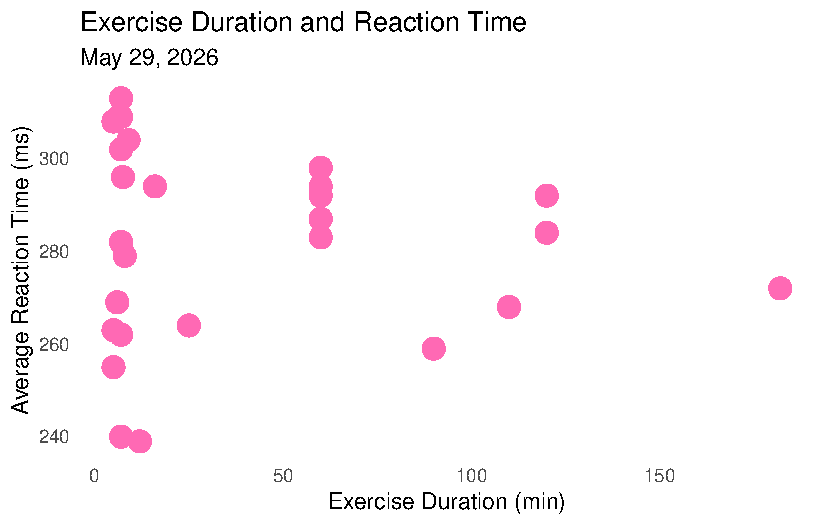
\includegraphics[keepaspectratio]{ENVS-193DS_homework-3_files/figure-pdf/unnamed-chunk-9-1.pdf}}

\subsection{b. Captions}\label{b.-captions}

\textbf{Figure 1. Mean reaction times across biking, volleyball, and
walking exercises.} Points represent observations of mean reaction time
(ms) after different kinds of exercise (pink: Biking, purple:
volleyball, blue: walking). Data from my personal observations. Data
accessed 2026-05-29.

\textbf{Figure 2. Mean reaction times and exercise duration.} Points
represent observations of mean reaction time (ms) in relation to
exercise duration (min). Data from my personal observations. Data
accessed 2026-05-29.

\section{Problem 3. Affective
visualization}\label{problem-3.-affective-visualization}

\subsection{a. Describe in words what an affective visualization could
look like for your personal
data.}\label{a.-describe-in-words-what-an-affective-visualization-could-look-like-for-your-personal-data.}

Taking inspiration from the Dear Data project, I could make a visual
where each observation is represented by an icon (a stick figure for
walking, a volleyball, and a bike tire for biking). Additional doodles
such as a water droplet or a star can indicate whether water was
consumed throughout exercise, or if an exercise exceeded a certain
amount of time. Colors can be used to indicate levels of social
interaction.

\subsection{b. Create a sketch (on paper) of your
idea.}\label{b.-create-a-sketch-on-paper-of-your-idea.}

\begin{figure}

\centering{

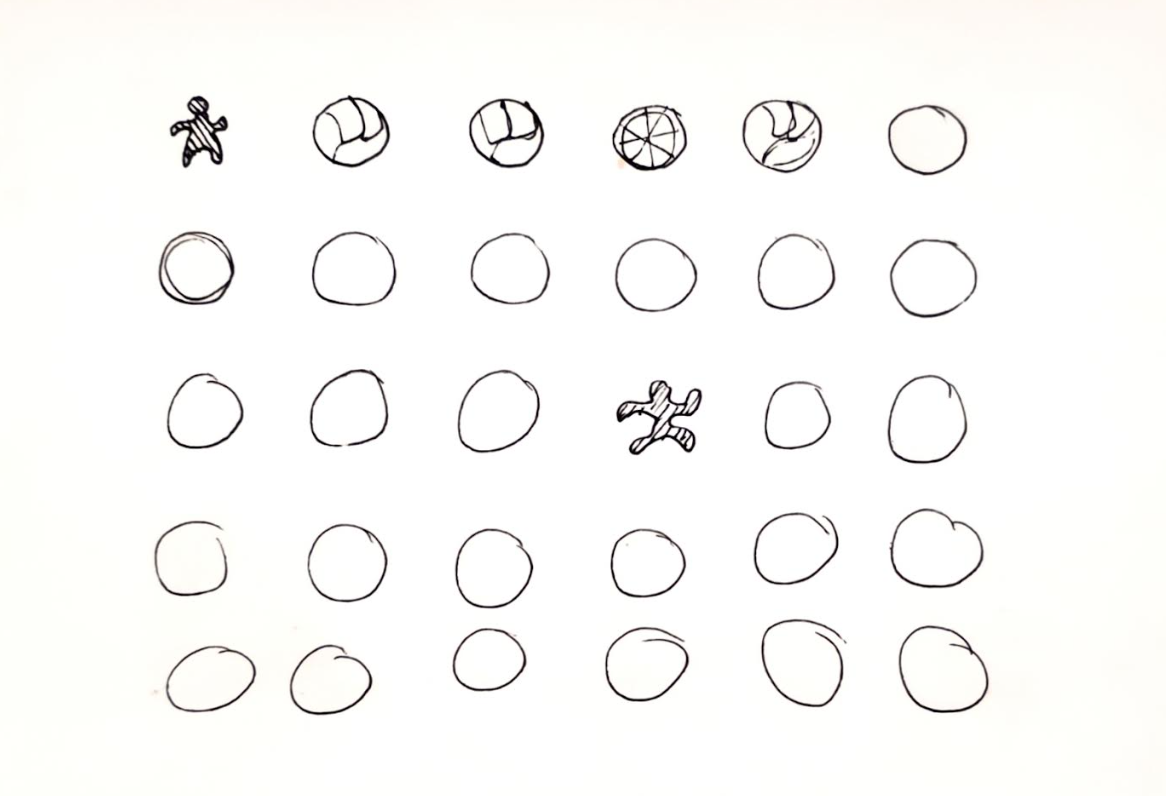
\includegraphics[width=4.16667in,height=\textheight,keepaspectratio]{../images/sketch.png}

}

\caption{\label{fig-screenshot-1}}

\end{figure}%

\subsection{c.~Make a draft of your
visualization.}\label{c.-make-a-draft-of-your-visualization.}

\begin{figure}

\centering{

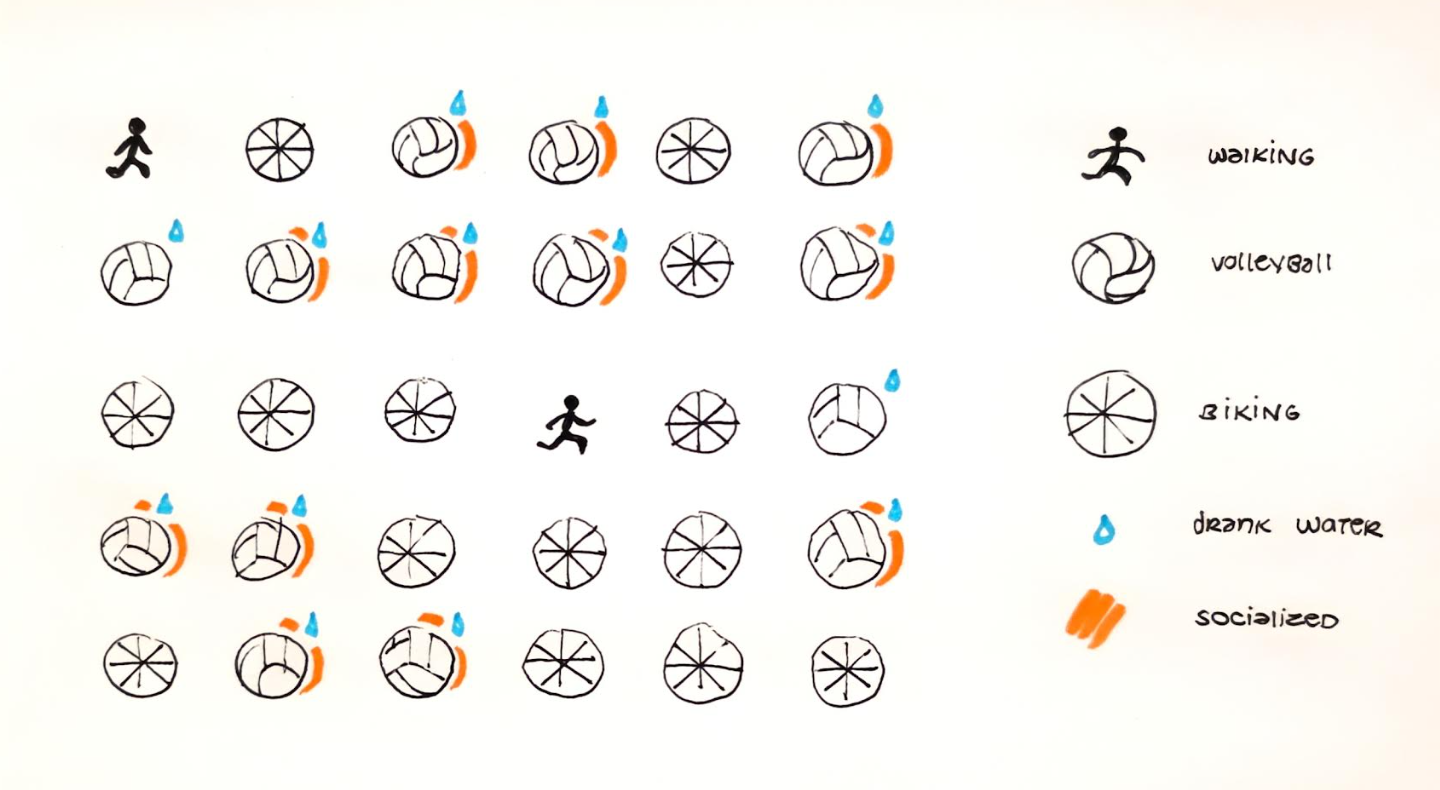
\includegraphics[width=4.16667in,height=\textheight,keepaspectratio]{../images/draft.png}

}

\caption{\label{fig-screenshot-2}}

\end{figure}%

\subsection{d.~Write an artist
statement.}\label{d.-write-an-artist-statement.}

This is a visualization of the exercises I have done throughout the
spring quarter. The icons arranged in an array of thirty observations
each represent a type of exercise (walking, biking, or volleyball) while
indicating factors such as socialization with other people and
hydration. I was inspired most by the Dear Data project; especially by
how colors and shapes were used not only to embellish the visualization
but to tell a story. I created this draft with a sheet of A4 paper, a
pen, and a couple highlighters. It is hand-drawn.

\subsection{e. Prep your materials to share in
class.}\label{e.-prep-your-materials-to-share-in-class.}

View presentation slides
\href{https://docs.google.com/presentation/d/1JCIGFIhqZ6NhE6zjIz3g13vsWye4e50MgZmk1uO-mqw/edit?usp=sharing}{here}.

\section{Problem 4. Statistical
critique}\label{problem-4.-statistical-critique}

\subsection{a. Revisit and summarize}\label{a.-revisit-and-summarize}

Pearson's R tests were used in this experiment to determine whether the
relationship between coral cover and sea urchin density across all six
studied reefs (Malindi, Watamu, Vipingo, Kanamai, Bamburi, and Diani)
was significant.

\begin{figure}

\centering{

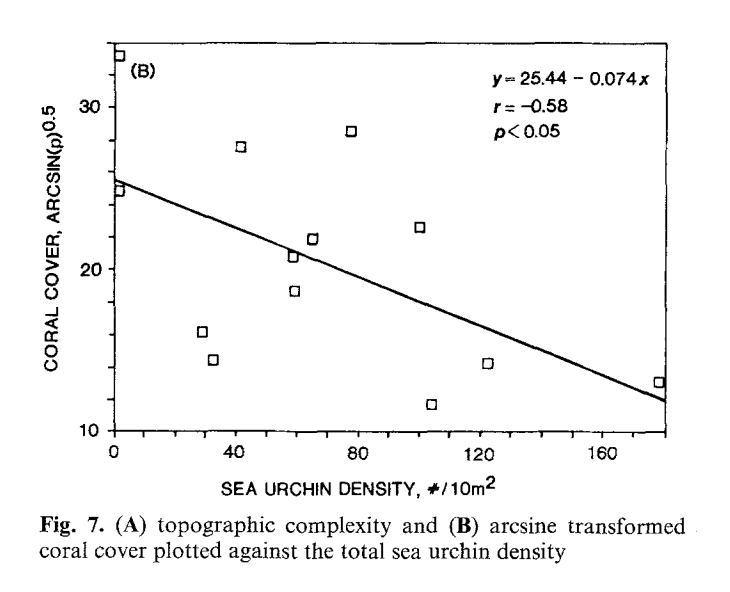
\includegraphics[width=4.16667in,height=\textheight,keepaspectratio]{../images/cc_sud.png}

}

\caption{\label{fig-screenshot-3}}

\end{figure}%

\subsection{b. Visual clarity}\label{b.-visual-clarity}

The statistics are clearly represented in this linear model; the x- and
y-axes are in logical positions while the line of best fit, the r-value,
p-value, model predictions (via the line of best fit), and underlying
data points are present.

\subsection{c.~Aesthetic clarity}\label{c.-aesthetic-clarity}

The data:ink ratio appears to be low. Visual clutter of the data is kept
to a minimum by only including values that are necessary to understand
it. This linear regression model is, structurally, quite neat as it is
used to display the relationship between two variables. There is a
slight sense of compaction, but that can be attributed to the
densely-packed nature of the paper itself.

\subsection{d.~Recommendations}\label{d.-recommendations}

I would try to further visually separate the variables (coral cover and
sea urchin density) from their units. Currently, they are separated by a
comma, which may be easily overlooked by quick eyes and potentially
confuse the reader. If this paper were to be made available not just in
black print, I think that the raw data and trend line would look
aesthetically pleasing in different colors (and allow them to stand out
visually from the rest of the figure).




\end{document}
